\textit{D3 is rigorously declarative, but not purely functional. Most of the work is done in stateful \say{function objects}, of which $\exists$ 4 main types:}\begin{itemize}
    \item Factory\textsubscript{F}: implement prescribed APIs
    \item Generator\textsubscript{G}: Generate concrete visualization code (SVG, Canvas) from passed data
    \item Layout\textsubscript{L}: Transform passed dataset to include additional visual layout information
    \item Component\textsubscript{C}: Manipulate the DOM
\end{itemize}\textit{Subscripts are used herein to categorize D3 functions according to the above taxonomy.}

\section{\href{https://github.com/d3/d3-selection}{Data Joining \& Selections}}

%%%%%%%%%%%%%%%%%%%%%%%%%%%%%%%%%%%%%%%%%%%%%%%%%%%
\subsec{\href{https://github.com/d3/d3-selection\#selecting-elements}{Selecting}}{\href{https://observablehq.com/@d3/selection-join}{d3}}
\textit{Create a \href{https://bost.ocks.org/mike/selection/}{selection} with one of the following top-level calls, generally passing a \href{http://www.w3.org/TR/selectors-api/}{W3C} selector string:}

{\footnotesize 
\begin{minipage}[t]{2.0cm}
    selection\\
    selector\\
    window
\end{minipage}
\begin{minipage}[t]{2.0cm}
    select\\
    selectorAll\\
    style
\end{minipage}
\begin{minipage}[t]{2.0cm}
    selectAll\\
    matcher\\
\end{minipage}
}



\textit{Create derivative selections (subsets, unions, \href{https://bost.ocks.org/mike/nest/}{nestings}) by invoking one of the following methods of an already-existing selection:}

{\footnotesize 
\begin{minipage}[t]{1.5cm}
    select
\end{minipage}
\begin{minipage}[t]{1.5cm}
    selectAll
\end{minipage}
\begin{minipage}[t]{1.5cm}
    filter
\end{minipage}
\begin{minipage}[t]{1.5cm}
    merge
\end{minipage}
}


%%%%%%%%%%%%%%%%%%%%%%%%%%%%%%%%%%%%%%%%%%%%%%%%%%%
\subsec{\href{https://github.com/d3/d3-selection\#modifying-elements}{Modifying}}{\href{https://observablehq.com/@d3/selection-join}{<selection>}}

\textit{Change properties of DOM elements in bulk:}

{\footnotesize 
\begin{minipage}[t]{2.0cm}
    attr\\
    text\\
    insert\\
    sort\\
    lower
\end{minipage}
\begin{minipage}[t]{2.0cm}
    classed\\
    html\\
    remove\\
    order\\
\end{minipage}
\begin{minipage}[t]{2.0cm}
    property\\
    append\\
    clone\\
    raise\\
\end{minipage}
}


%%%%%%%%%%%%%%%%%%%%%%%%%%%%%%%%%%%%%%%%%%%%%%%%%%%
\subsec{\href{https://github.com/d3/d3-selection\#joining-data}{Joining}}{\href{http://bost.ocks.org/mike/join/}{<selection>}}

\href{https://bost.ocks.org/mike/circles/}{\resizebox{4cm}{!}{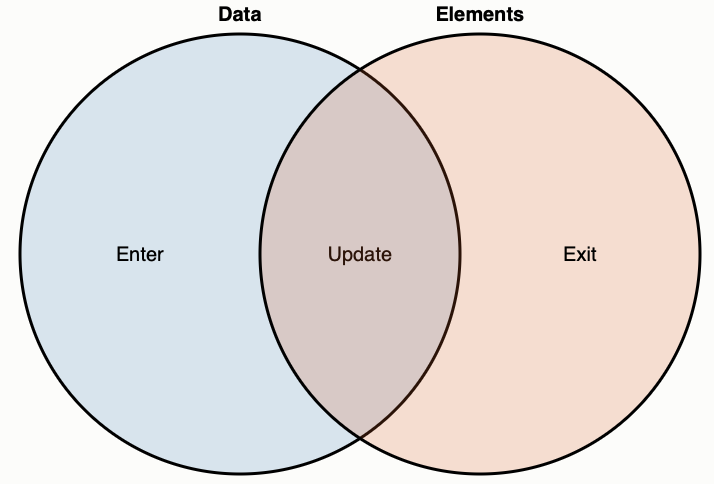
\includegraphics[]{img/gup.png}}}

\textit{The \href{https://bost.ocks.org/mike/join/}{\say{General Update Pattern}} involves a \say{data join}, followed by references to the resulting subset of elements \& data, and looks something like this:}

\code{svg.selectAll(\textquotedbl circle\textquotedbl)}\\
\code{\phantom{xx}.data(data)}\\
\code{\phantom{xx}.enter().append(\textquotedbl circle\textquotedbl)}\\
\code{\phantom{xxxx}.attr(\textquotedbl cx\textquotedbl , function(d) \{ return d.x; \})}\\
\code{\phantom{xxxx}.attr(\textquotedbl cy\textquotedbl , function(d) \{ return d.y; \})}\\
\code{\phantom{xxxx}.attr(\textquotedbl r\textquotedbl , 2.5);}\\

{\footnotesize 
\begin{minipage}[t]{1.2cm}
    data
\end{minipage}
\begin{minipage}[t]{1.2cm}
    join
\end{minipage}
\begin{minipage}[t]{1.2cm}
    enter
\end{minipage}
\begin{minipage}[t]{1.2cm}
    exit
\end{minipage}
\begin{minipage}[t]{1.2cm}
    datum
\end{minipage}
}

%%%%%%%%%%%%%%%%%%%%%%%%%%%%%%%%%%%%%%%%%%%%%%%%%%%
\subsec{\href{https://github.com/d3/d3-selection\#handling-events}{Events}}{d3}

\textit{Add/remove an event-handler with }\texttt{<selection>.on()}\textit{, or immediately dispatch an event with }\texttt{<selection>.dispatch()}\textit{. The following top-level functions return information about an active event:}

{\footnotesize 
\begin{minipage}[t]{2.0cm}
    event\\
    touch
\end{minipage}
\begin{minipage}[t]{2.0cm}
    customEvent\\
    touches
\end{minipage}
\begin{minipage}[t]{2.0cm}
    mouse\\
    clientPoint
\end{minipage}
}



%%%%%%%%%%%%%%%%%%%%%%%%%%%%%%%%%%%%%%%%%%%%%%%%%%%
\subsec{\href{https://github.com/d3/d3-selection\#control-flow}{Control}}{<selection>}

\textit{The following yield information about selections, except for }\texttt{each}\textit{ and }\texttt{call}\textit{, which afford arbitrary code execution for selections while maintaining the ability to chain subsequent methods.}


{\footnotesize 
\begin{minipage}[t]{2.0cm}
    each\\
    nodes
\end{minipage}
\begin{minipage}[t]{2.0cm}
    call\\
    node
\end{minipage}
\begin{minipage}[t]{2.0cm}
    empty\\
    size
\end{minipage}
}


%%%%%%%%%%%%%%%%%%%%%%%%%%%%%%%%%%%%%%%%%%%%%%%%%%%
\subsec{\href{https://github.com/d3/d3-selection\#local-variables}{Local Variables}}{\href{http://bl.ocks.org/mbostock/e1192fe405703d8321a5187350910e08}{<selection>}}

\textit{Afford the storage/retrieval of state that is independent of a selection\textquotesingle s data.}

{\footnotesize 
\begin{minipage}[t]{1.5cm}
    set
\end{minipage}
\begin{minipage}[t]{1.5cm}
    get
\end{minipage}
\begin{minipage}[t]{1.5cm}
    remove
\end{minipage}
\begin{minipage}[t]{1.5cm}
    toString
\end{minipage}
}


%%%%%%%%%%%%%%%%%%%%%%%%%%%%%%%%%%%%%%%%%%%%%%%%%%%
\subsec{Namespaces}{d3}

\textit{For use in construction XML namespaces.}

{\footnotesize 
\begin{minipage}[t]{2.0cm}
    namespace
\end{minipage}
\begin{minipage}[t]{2.0cm}
    namespaces
\end{minipage}
}
